\chapter{RTS Smoother}
\label{ch:rts}

The tracker described in Chapter~\ref{ch:tracking} is a causal filter, i.e.\ the estimate
at each instant is computed only from the measurements received up to that instant. This
limits the quality of the estimate during the maneuvers. The CCA model assumes a constant
acceleration over each prediction interval, while on track the opponent alternates
braking, cornering and traction phases, in which the acceleration changes abruptly. In
these phases the filter can only follow the new dynamics after the measurements have shown
it, and the estimate lags behind the true state of the opponent.

An alternative approach to improve the quality of the estimate of the state of the
opponent during the maneuvers is presented in this chapter, and consists in the
implementation of an acausal filter. The idea is to exploit the future information, i.e.\
the measurements acquired after each instant, to refine the estimate of the past states of
the opponent. This is the purpose of a smoother, an acausal estimator that computes the
state at each instant from the measurements acquired both before and after it.

This choice is also made possible by the fact that, in the application, the estimate of
the opponent is used by the planning module to perform the gap control, i.e.\ to regulate
the distance from the opponent in terms of time. For this purpose, the real-time estimate
of the state of the opponent is not strictly necessary, and a past estimate can also be
used, provided that it is more accurate.

Specifically, among the smoothing algorithms, the Rauch--Tung--Striebel (RTS) smoother is
adopted. It comes in handy since it reuses the causal estimate of the Kalman filter and
enhances it with a backward recursion, so that it can be added to the existing tracker
without modifying it.

Section~\ref{sec:rts_problem} introduces the smoothing problem and its relation with
filtering and prediction. Section~\ref{sec:rts_formulation} derives the RTS smoother and its application on a
sliding window of the history.
Section~\ref{sec:rts_implementation} describes its implementation in the target tracking
module. Finally, Section~\ref{sec:rts_sensitivity} analyzes the effect of the window
length on the smoothed estimate, with and without the RaDAR measurements.

% =====================================================================
\section{From Filtering to Smoothing}
\label{sec:rts_problem}

Given the set of measurements $\mathbf{Y}_N = \{\mathbf{z}_1, \dots, \mathbf{z}_N\}$, the
estimate of the state $\mathbf{x}_k$ at instant $k$ is the value that maximizes the
conditional probability density of the state given the measurements,
\begin{equation}
    \hat{\mathbf{x}}_{k|N} = \arg\max_{\mathbf{x}_k}\; p\left(\mathbf{x}_k \mid \mathbf{Y}_N\right).
    \label{eq:rts_map}
\end{equation}
Depending on the relation between $k$ and the last measurement $N$, three problems are
distinguished.
\begin{itemize}
    \item \textbf{Prediction}, with $N < k$, in which the measurements stop before the
    instant of interest and the state is extrapolated through the model.
    \item \textbf{Filtering}, with $N = k$, in which the measurements are available up to
    the instant of interest. This is the problem solved by the Kalman filter.
    \item \textbf{Smoothing}, with $N > k$, in which also the measurements acquired after
    the instant of interest are used.
\end{itemize}
The three problems share the same conditional density, and only the information used to
compute it changes. The Kalman filter, introduced in 1960, solves the filtering problem.
In 1965, Rauch, Tung and Striebel showed that the smoothing problem can be solved from
the same principle, i.e.\ the maximization of the likelihood, and in a recursive form,
which runs backward on the output of the Kalman filter.

An alternative solution is given by the two-filter approach of Fraser and Potter, in
which the smoothed estimate is obtained as the combination of two Kalman filters, one
running forward from the first measurement and one running backward from the last one.
The two formulations have been proven to be equivalent. In this work, the RTS formulation is chosen since it is more convenient
from an implementation point of view. It exploits the quantities already computed by the
forward filter, which only have to be stored, and it is lighter, since it does not require
a second filter running in parallel, with its own initialization. The backward recursion
is instead initialized with the estimate of the forward filter at the current time.

% =====================================================================
\section{RTS Smoother Formulation}
\label{sec:rts_formulation}

The derivation is first presented for a linear system,
\begin{equation}
    \mathbf{x}_{k+1} = \mathbf{F}_k\,\mathbf{x}_k + \mathbf{w}_k,
    \qquad
    \mathbf{z}_k = \mathbf{H}_k\,\mathbf{x}_k + \mathbf{v}_k,
    \label{eq:rts_linear}
\end{equation}
with $\mathbf{w}_k$ and $\mathbf{v}_k$ zero-mean Gaussian white noises with covariance
$\mathbf{Q}_k$ and $\mathbf{R}_k$. For the EKF of the tracker, $\mathbf{F}_k$ is the
Jacobian~\eqref{eq:tt_F} of the motion model, evaluated at the filtered estimate.

\subsection{Forward Pass}
\label{subsec:rts_forward}

The forward pass is the Kalman filter of Chapter~\ref{ch:tracking}. At each step, the
state is predicted,
\begin{equation}
    \hat{\mathbf{x}}_{k+1|k} = \mathbf{F}_k\,\hat{\mathbf{x}}_{k|k},
    \qquad
    \mathbf{P}_{k+1|k} = \mathbf{F}_k\,\mathbf{P}_{k|k}\,\mathbf{F}_k^\top + \mathbf{Q}_k,
    \label{eq:rts_fwd_pred}
\end{equation}
and then corrected with the measurement,
\begin{equation}
    \begin{aligned}
        \mathbf{K}_{k+1} &= \mathbf{P}_{k+1|k}\,\mathbf{H}_{k+1}^\top
        \left(\mathbf{H}_{k+1}\,\mathbf{P}_{k+1|k}\,\mathbf{H}_{k+1}^\top + \mathbf{R}_{k+1}\right)^{-1}, \\
        \hat{\mathbf{x}}_{k+1|k+1} &= \hat{\mathbf{x}}_{k+1|k}
        + \mathbf{K}_{k+1}\left(\mathbf{z}_{k+1} - \mathbf{H}_{k+1}\,\hat{\mathbf{x}}_{k+1|k}\right),
    \end{aligned}
    \label{eq:rts_fwd_corr}
\end{equation}
as in~\eqref{eq:tt_prediction} and~\eqref{eq:tt_update}. For the backward step, the
prior estimate $\hat{\mathbf{x}}_{k+1|k}$ and its covariance $\mathbf{P}_{k+1|k}$ are
stored at every step, together with the state matrix $\mathbf{F}_k$, to compute the
smoothed estimate.

\subsection{Backward Recursion}
\label{subsec:rts_backward}

The backward recursion is derived from the joint probability density of two consecutive
states and of the measurements, $p(\mathbf{x}_k, \mathbf{x}_{k+1}, \mathbf{Y}_N)$.
Applying the Markov property of the model, i.e.\ once $\mathbf{x}_{k+1}$ is given the
future measurements $\mathbf{z}_{k+1}, \dots, \mathbf{z}_N$ do not depend on
$\mathbf{x}_k$, the density can be factorized as
\begin{equation}
    p(\mathbf{x}_k, \mathbf{x}_{k+1}, \mathbf{Y}_N) =
    p(\mathbf{z}_{k+1}, \dots, \mathbf{z}_N \mid \mathbf{x}_{k+1})\;
    p(\mathbf{x}_{k+1} \mid \mathbf{x}_k)\;
    p(\mathbf{x}_k \mid \mathbf{Y}_k)\;
    p(\mathbf{Y}_k),
    \label{eq:rts_joint}
\end{equation}
This factorization links the step $k$ to the step $k+1$, whose smoothed estimate is
already available from the previous backward step, and is the origin of the recursion.
In~\eqref{eq:rts_joint}, only the second and the third terms depend on $\mathbf{x}_k$.
Both are Gaussian, the first with mean $\mathbf{F}_k\,\mathbf{x}_k$ and covariance
$\mathbf{Q}_k$, the second with mean $\hat{\mathbf{x}}_{k|k}$ and covariance
$\mathbf{P}_{k|k}$, given by the forward pass. Taking the logarithm, the smoothed estimate
$\hat{\mathbf{x}}_{k|N}$ is the value that minimizes the cost function
\begin{equation}
    J(\mathbf{x}_k) =
    \left\|\hat{\mathbf{x}}_{k+1|N} - \mathbf{F}_k\,\mathbf{x}_k\right\|^2_{\mathbf{Q}_k^{-1}}
    + \left\|\mathbf{x}_k - \hat{\mathbf{x}}_{k|k}\right\|^2_{\mathbf{P}_{k|k}^{-1}},
    \label{eq:rts_cost}
\end{equation}
in which $\mathbf{x}_{k+1}$ has been replaced by its smoothed estimate. The cost function
contains two terms. The first measures the consistency with the future, i.e.\ the mismatch
between the smoothed state at $k+1$ and the prediction propagated from $\mathbf{x}_k$,
weighted by the inverse of the process noise covariance. The second measures the
consistency with the past, i.e.\ the distance from the filtered estimate, weighted by the
inverse of its covariance. Setting the gradient of $J$ to zero and applying the matrix
inversion lemma gives the smoother gain
\begin{equation}
    \mathbf{C}_k = \mathbf{P}_{k|k}\,\mathbf{F}_k^\top
    \left(\mathbf{F}_k\,\mathbf{P}_{k|k}\,\mathbf{F}_k^\top + \mathbf{Q}_k\right)^{-1}
    = \mathbf{P}_{k|k}\,\mathbf{F}_k^\top\,\mathbf{P}_{k+1|k}^{-1},
    \label{eq:rts_gain}
\end{equation}
the smoothed estimate
\begin{equation}
    \hat{\mathbf{x}}_{k|N} = \hat{\mathbf{x}}_{k|k}
    + \mathbf{C}_k\left(\hat{\mathbf{x}}_{k+1|N} - \hat{\mathbf{x}}_{k+1|k}\right),
    \label{eq:rts_state}
\end{equation}
and its covariance
\begin{equation}
    \mathbf{P}_{k|N} = \mathbf{P}_{k|k}
    + \mathbf{C}_k\left(\mathbf{P}_{k+1|N} - \mathbf{P}_{k+1|k}\right)\mathbf{C}_k^\top.
    \label{eq:rts_cov}
\end{equation}

The smoother gain has the same structure as the Kalman gain in~\eqref{eq:rts_fwd_corr},
with the substitution of $\mathbf{H}_{k+1}$ with $\mathbf{F}_k$, of $\mathbf{R}_{k+1}$ with
$\mathbf{Q}_k$ and of $\mathbf{P}_{k+1|k}$ with $\mathbf{P}_{k|k}$. In the Kalman filter,
the measurement corrects the predicted state. In the smoother, the smoothed state at
$k+1$ acts as a pseudo-measurement that corrects the filtered state at $k$.

The correction of the acausal state depends on two factors. The first is the mismatch
between the prediction $\hat{\mathbf{x}}_{k+1|k}$ and the smoothed state
$\hat{\mathbf{x}}_{k+1|N}$. If the model is correct, the mismatch is small and the
smoothed state remains close to the causal one. If instead the dynamics of the opponent
has changed, e.g.\ at the beginning of a maneuver, the smoothed state differs from the
prediction and the mismatch is larger. The mismatch is then weighted by the gain
$\mathbf{C}_k$, which incorporates the uncertainty of the filter through
$\mathbf{P}_{k|k}$. If the filter is not very uncertain, the gain is small and the
smoother corrects little, since the filtered estimate does not need the future
information. If the filter is uncertain, the gain is larger and the future information
weighs more on the smoothed estimate.

The recursion is initialized at the last step, $k = N$, where the measurements used by
the filter and by the smoother coincide, so that the filtered estimate
$\hat{\mathbf{x}}_{N|N}$ and its covariance $\mathbf{P}_{N|N}$ are also the smoothed
ones. The recursion~\eqref{eq:rts_gain}--\eqref{eq:rts_cov} is then applied backward, for
$k = N-1, \dots, 0$.

\subsection{Fixed-Lag Smoothing on a Sliding Window}
\label{subsec:rts_window}

The formulation above refers to a fixed interval, in which all the measurements are
available before the backward pass starts. In the tracker, the measurements keep
arriving, and the smoother is applied on a sliding window of duration $T_w$, which
contains the steps to be smoothed, between $t_N - T_w$ and the most recent one $t_N$. The
smoother acts on the history of the opponent that is passed to the planning module. At
every publication, the backward pass is run on the whole window, starting from the most
recent step. As the window slides, each past state is smoothed again with the newly
available measurements, and its estimate is progressively refined. The estimate of a
state at a time $d$ before the most recent step, here referred to as buffer age, is
obtained with $d$ seconds of future measurements, so that the buffer age plays the role of
the lag of a fixed-lag smoother. The complete algorithm is reported in
Algorithm~\ref{alg:rts}.

\begin{algorithm}[H]
\caption{RTS smoother on the sliding window of the history, for a single track.}
\label{alg:rts}
\begin{algorithmic}[1]
\REQUIRE entries $k = 0, \dots, N$ of the history of the track in the window
$[t_N - T_w,\, t_N]$, storing $\hat{\mathbf{x}}_{k|k}$, $\mathbf{P}_{k|k}$,
$\hat{\mathbf{x}}_{k+1|k}$, $\mathbf{P}_{k+1|k}$ and $\mathbf{F}_k$
\ENSURE smoothed estimates $\hat{\mathbf{x}}_{k|N}$ and $\mathbf{P}_{k|N}$
\IF{the smoother is disabled \OR $N < 1$}
    \RETURN the causal estimates
\ENDIF
\STATE $\hat{\mathbf{x}}_{N|N},\, \mathbf{P}_{N|N} \leftarrow$ filtered estimate \COMMENT{initialization}
\FOR{$k = N-1$ \textbf{down to} $0$}
    \IF{the prediction $\hat{\mathbf{x}}_{k+1|k}$, $\mathbf{P}_{k+1|k}$ is stored}
        \STATE $\mathbf{C}_k \leftarrow \mathbf{P}_{k|k}\,\mathbf{F}_k^\top\,\mathbf{P}_{k+1|k}^{-1}$
        \STATE $\hat{\mathbf{x}}_{k|N} \leftarrow \hat{\mathbf{x}}_{k|k} + \mathbf{C}_k\left(\hat{\mathbf{x}}_{k+1|N} - \hat{\mathbf{x}}_{k+1|k}\right)$
        \STATE $\mathbf{P}_{k|N} \leftarrow \mathbf{P}_{k|k} + \mathbf{C}_k\left(\mathbf{P}_{k+1|N} - \mathbf{P}_{k+1|k}\right)\mathbf{C}_k^\top$
    \ELSE
        \STATE $\hat{\mathbf{x}}_{k|N},\, \mathbf{P}_{k|N} \leftarrow$ filtered estimate \COMMENT{causal fallback}
    \ENDIF
\ENDFOR
\RETURN $\hat{\mathbf{x}}_{k|N}$, $\mathbf{P}_{k|N}$ for $k = 0, \dots, N$
\end{algorithmic}
\end{algorithm}

% =====================================================================
\section{Implementation}
\label{sec:rts_implementation}

The smoother is implemented as a read-only layer on top of the causal filter. It never
writes back into the EKF, so that the forward pass, the life cycle of the tracks and the
current state published to the planning module remain unchanged. The smoothed states are
stored alongside the causal ones, and the smoother can be disabled through a parameter,
which restores the original behavior of the tracker.

The smoother relies on the history of the tracker already introduced for the
out-of-sequence measurements (Section~\ref{subsec:tt_oosm}), in which each entry contains
the state of all the tracks after the processing of a measurement. In the prediction step
of the EKF, right after the propagation and before the correction, the predicted state
$\hat{\mathbf{x}}_{k+1|k}$, its covariance $\mathbf{P}_{k+1|k}$ and the Jacobian
$\mathbf{F}_k$ are stored in the track, so that each entry of the history contains all the
quantities required by the backward pass.

At every publication, the window $[t_N - T_w,\, t_N]$ is extracted from the history, with
$t_N$ the time of the most recent entry, and at least two entries are required to run the
smoother. The backward pass then pairs each entry $k$ with the following one $k+1$, and
for each track of entry $k$ looks for the same track in entry $k+1$. The future state is
the one smoothed at the previous iteration or, when it is not available, the causal one.
Only the state and the covariance are replaced by the smoothed ones, while the other
fields of the track, such as its identifier and timestamp, are copied from the causal
estimate. Every degenerate case, such as a track that has just been initialized or a state
without future support, falls back to the causal estimate, so that the output is always
complete.

The implementation is also robust to the out-of-sequence measurements. When a late
measurement arrives, the tracker inserts it in the history according to its acquisition
time and reprocesses all the following entries (Section~\ref{subsec:tt_oosm}), so that
the filtered states, the predictions and the Jacobians stored in the history are updated.
Since the smoother never modifies the history and recomputes the whole window from the
stored quantities at every publication, the late measurement is automatically included
in the next backward pass, and no smoothed state has to be corrected or invalidated.

The history published to the planning module contains, at the current time, the causal
prediction of the Kalman filter, without any correction. From the first available
measurement backward, it contains the smoothed history, using the smoothed state when it
is available and the causal one otherwise. In this way, the most recent state of the
opponent is published without any additional delay, and its past states benefit from the
future measurements.

% =====================================================================
\section{Sensitivity Analysis}
\label{sec:rts_sensitivity}

The main parameter of the smoother is the window length $T_w$, which sets how much future
information is available to smooth each state. In the following, the estimates are
compared at different window lengths, i.e.\ at different buffer ages, where a window of
\SI{0}{ms} corresponds to the most recent filtered estimate, i.e.\ the correction, and a
negative window to the causal prediction at the publication time. The effect of the
window is evaluated on the speed of the opponent, compared with the ground truth through
two metrics.
\begin{itemize}
    \item \textbf{RMSE of the speed}, computed between the estimate at a given window
    length and the ground truth at the corresponding time, both on the whole session
    (global RMSE) and on the braking phases only (local RMSE).
    \item \textbf{Maneuver delay}, i.e.\ the time difference between the instant at which the
    estimated speed starts a braking maneuver and the same instant for the ground truth. A
    positive value indicates that the estimate starts the maneuver late, a negative one
    that it anticipates it. The braking maneuvers are identified on the ground truth, 63
    in the session analyzed, and the delay is summarized by its median over the
    maneuvers for which the start of the braking is detected in the estimate, i.e.\ 49
    with all the sensors and 44 without the RaDAR.
\end{itemize}

The window length is analyzed on the session recorded on the day of the race at Imola, on
5 September 2026. The sensitivity analysis is carried out first with the measurements of
all the sensors, and then removing the measurements of the RaDAR, i.e.\ the measurement of
the speed. With all the sensors, Fig.~\ref{fig:rts_lag_radar} shows the speed of the
opponent during a braking phase and a full corner. The prediction is the causal estimate
of the filter at the publication time, the correction is the most recent filtered
estimate, and the other curves are the smoothed estimates obtained with windows from 100
to \SI{500}{ms}. As the window increases, the smoothed estimate moves closer to the
ground truth, both at the beginning of the braking and around the apex of the corner. With
the RaDAR, the curves obtained with windows longer than about \SI{200}{ms} are almost
superimposed.

\begin{figure}[!htbp]
    \centering
    \subfloat[Braking]{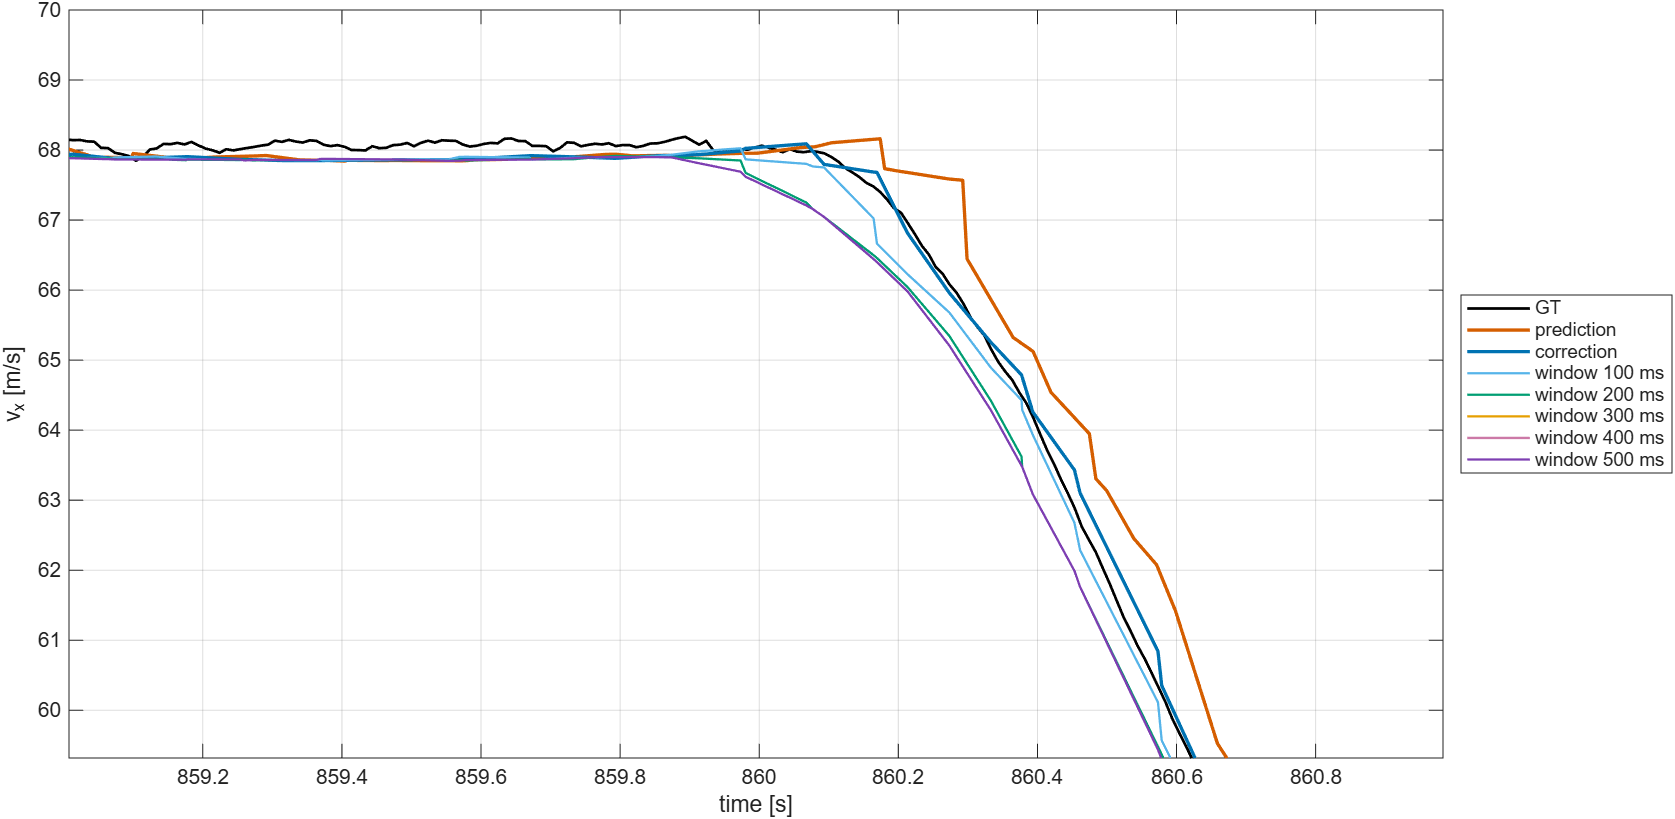
\includegraphics[width=0.76\textwidth]{figures/ch6/rts_lag_radar_braking.png}}\\
    \subfloat[Corner]{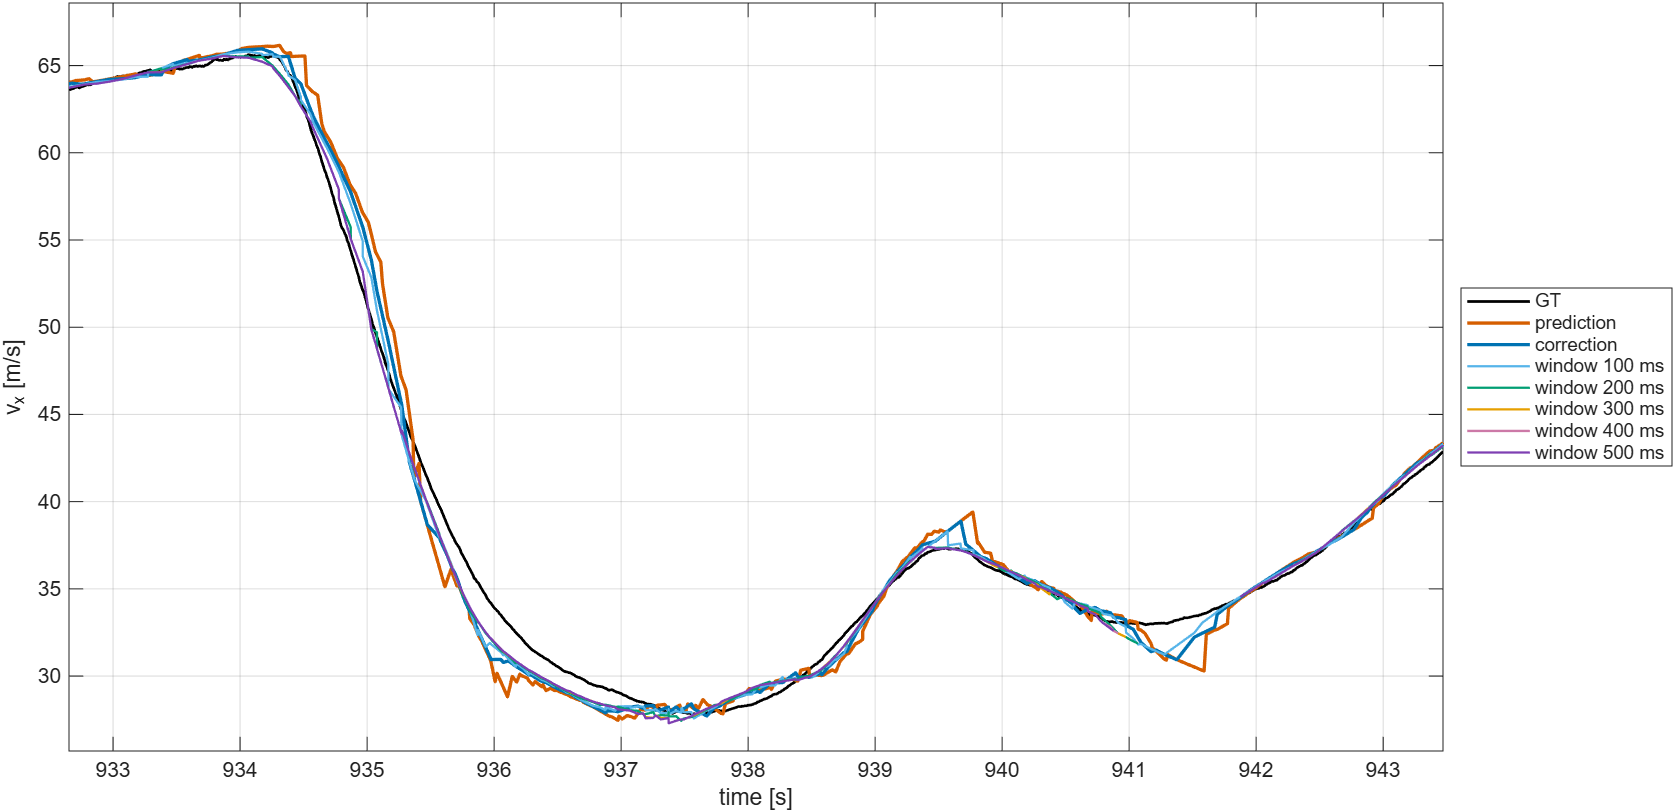
\includegraphics[width=0.76\textwidth]{figures/ch6/rts_lag_radar_corner.png}}
    \caption{Speed of the opponent estimated with different windows, all the sensors.}
    \label{fig:rts_lag_radar}
\end{figure}

The RMSE and the maneuver delay as a function of the window length are shown in
Fig.~\ref{fig:rts_metrics_radar} and reported in Table~\ref{tab:rts_radar}. With all the
sensors, increasing the window improves the estimate up to about 200--\SI{300}{ms}, beyond
which the gain saturates. With respect to the filtered estimate, the global RMSE decreases
by \SI{31}{\percent} and the local one by \SI{35}{\percent}. The saturation is due to the
fact that the forward filter already has a direct measurement of the speed, i.e.\ the
range rate of the RaDAR. The filter is therefore not very uncertain and, as discussed in
Section~\ref{subsec:rts_backward}, it does not need many future measurements. The median
maneuver delay moves from $+19$\,ms for the filtered estimate to about \SI{-62}{ms} for
windows longer than about \SI{180}{ms}, i.e.\ the smoothed estimate starts the maneuver
slightly before the ground truth. This anticipation is a direct consequence of the
backward pass. The future measurements that reveal the maneuver are spread backward over
the window, so that the estimate starts moving towards the new state before the maneuver
actually starts.

\begin{figure}[!htbp]
    \centering
    \subfloat[RMSE of the speed]{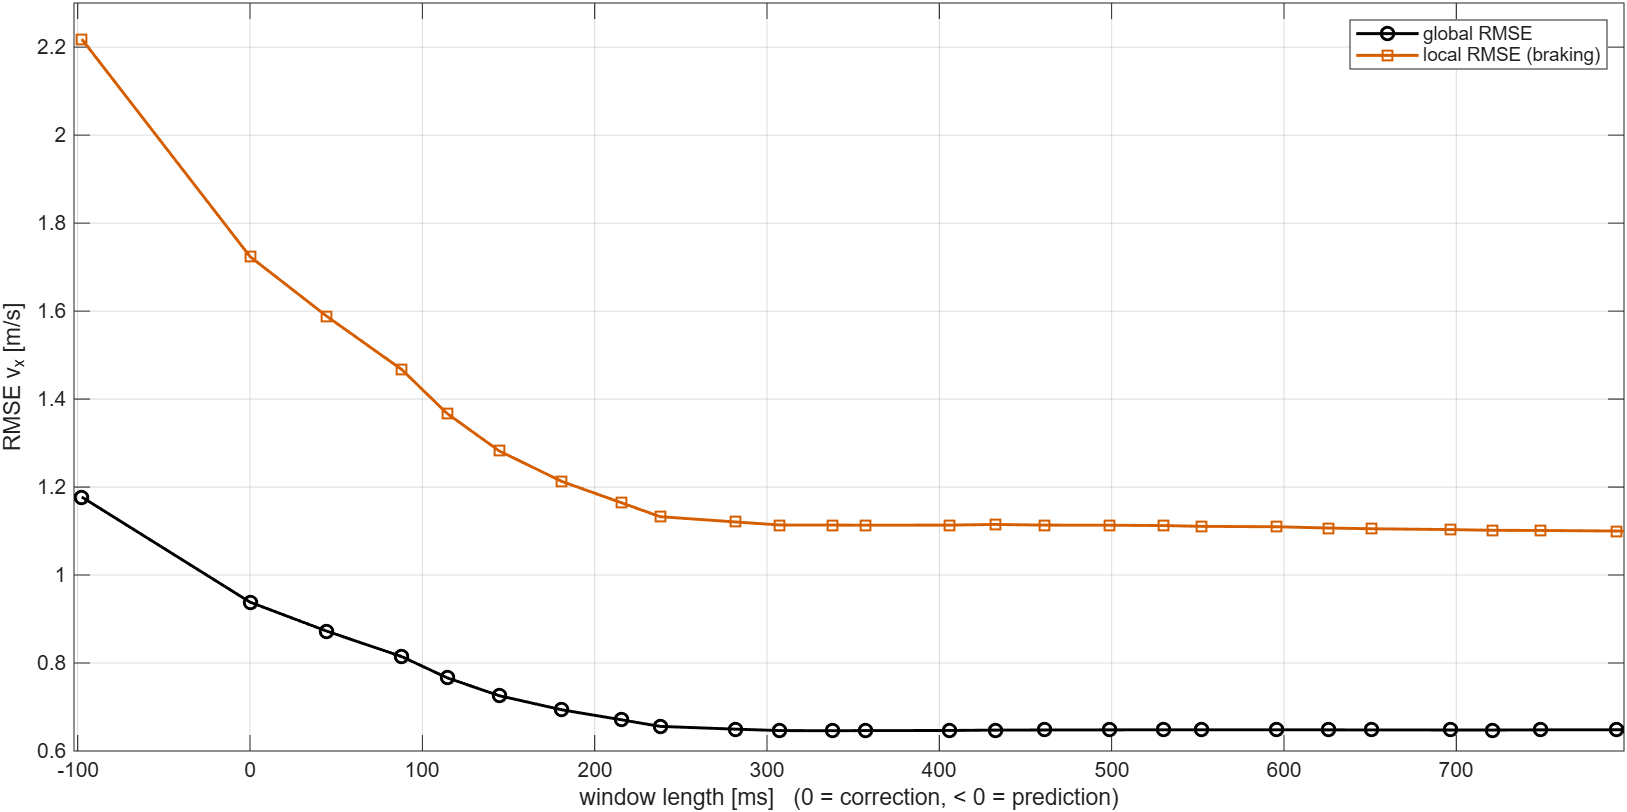
\includegraphics[width=0.76\textwidth]{figures/ch6/rts_rmse_radar.png}}\\
    \subfloat[Maneuver delay]{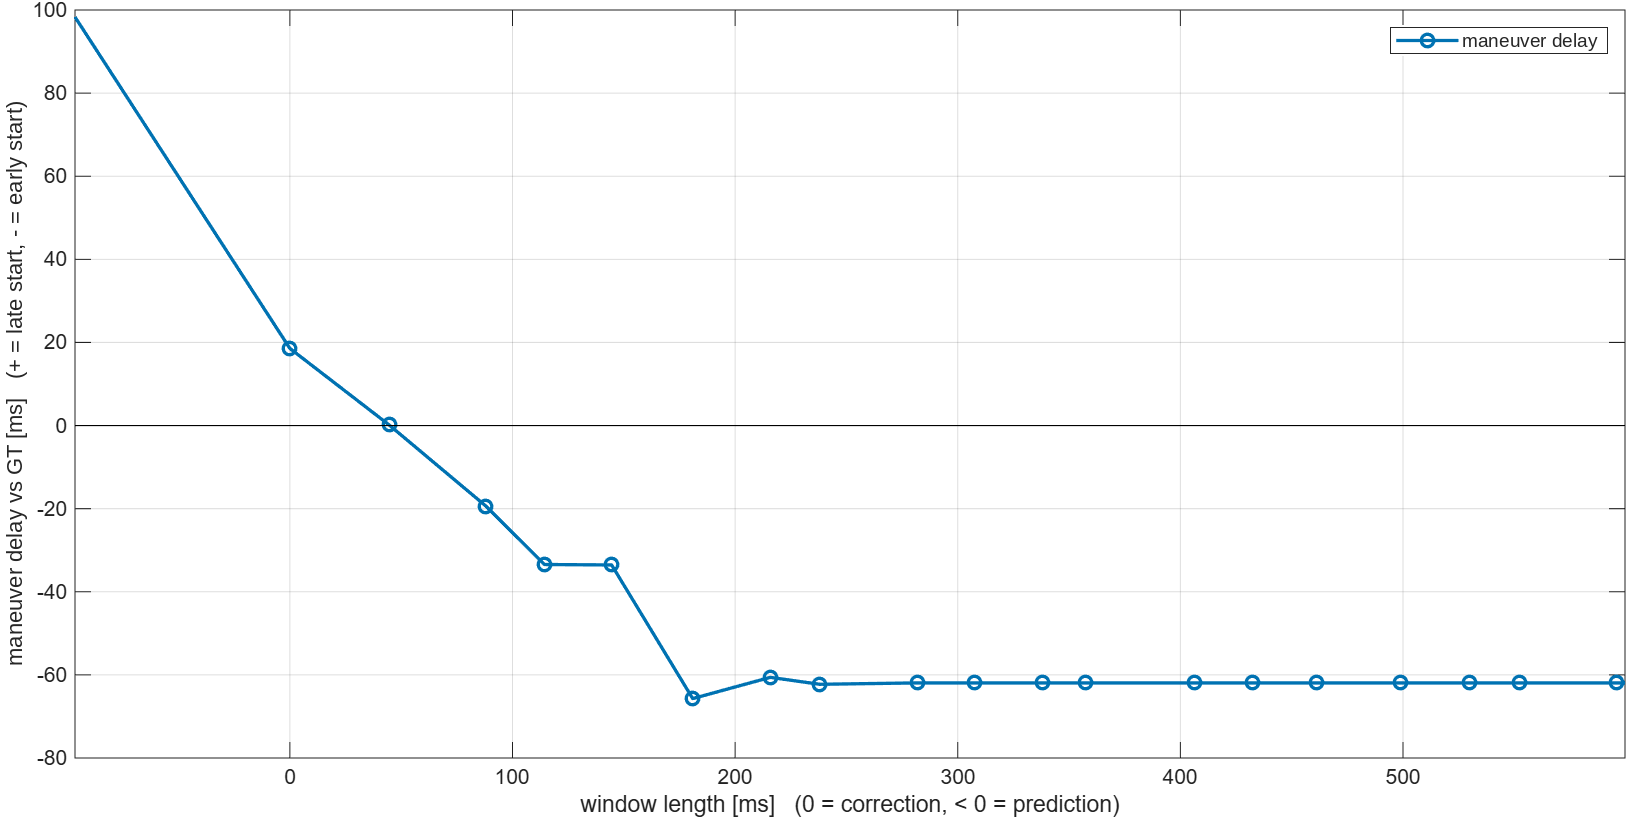
\includegraphics[width=0.76\textwidth]{figures/ch6/rts_delay_radar.png}}
    \caption{RMSE of the speed and maneuver delay as a function of the window length, all the
    sensors.}
    \label{fig:rts_metrics_radar}
\end{figure}

\begin{table}[!htbp]
\centering
\small
\begin{tabular}{rccccc}
\toprule
Window & \multicolumn{2}{c}{Global RMSE} & \multicolumn{2}{c}{Local RMSE} & Maneuver delay \\
\cmidrule(lr){2-3}\cmidrule(lr){4-5}
[ms] & [m/s] & $\Delta$ [\%] & [m/s] & $\Delta$ [\%] & [ms] \\
\midrule
  $-98$ & 1.177 & $+25.5$ & 2.218 & $+28.7$ & $+99$ \\
      0 & 0.938 & -- & 1.724 & -- & $+19$ \\
     88 & 0.815 & $-13.1$ & 1.467 & $-14.9$ & $-19$ \\
    145 & 0.726 & $-22.6$ & 1.282 & $-25.6$ & $-34$ \\
    216 & 0.671 & $-28.5$ & 1.164 & $-32.5$ & $-61$ \\
    308 & 0.646 & $-31.1$ & 1.114 & $-35.4$ & $-62$ \\
    406 & 0.647 & $-31.0$ & 1.113 & $-35.4$ & $-62$ \\
    499 & 0.648 & $-30.9$ & 1.113 & $-35.4$ & $-62$ \\
    697 & 0.648 & $-30.9$ & 1.103 & $-36.0$ & $-62$ \\
   1015 & 0.651 & $-30.6$ & 1.103 & $-36.0$ & $-62$ \\
\bottomrule
\end{tabular}
\caption{RMSE of the speed and median maneuver delay as a function of the window length, all the sensors. $\Delta$ is the variation with respect to the filtered estimate.}
\label{tab:rts_radar}
\end{table}

\FloatBarrier
\subsection*{Without Speed Measurements}
\label{subsec:rts_radar}

When the direct measurement of the speed is removed, i.e.\ without the RaDAR, the result
becomes more interesting. The speed is reconstructed from the positions only, the forward
filter is more uncertain, and the smoother corrects more. Fig.~\ref{fig:rts_lag_noradar}
shows that, in this case, the prediction and the correction lag behind the ground truth
more evidently, and the smoothed estimates obtained with the different windows are now
clearly separated. The longer the window, the earlier the smoothed estimate follows the
braking, until, for the longest windows, it starts the maneuver before the ground truth.

\begin{figure}[!htbp]
    \centering
    \subfloat[Braking]{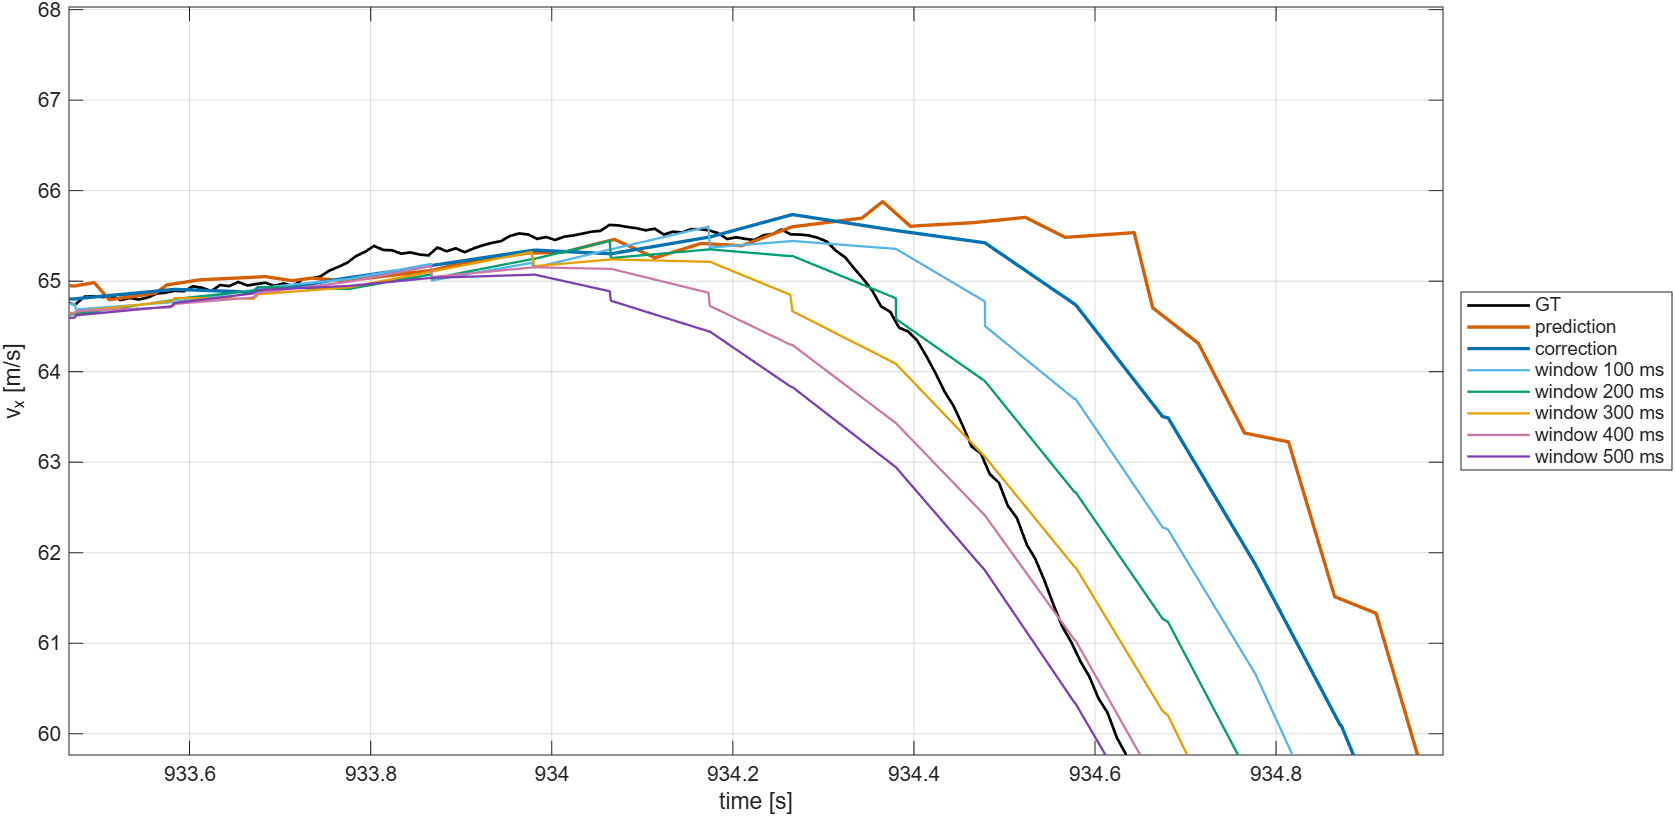
\includegraphics[width=0.76\textwidth]{figures/ch6/rts_lag_noradar_braking.png}}\\
    \subfloat[Corner]{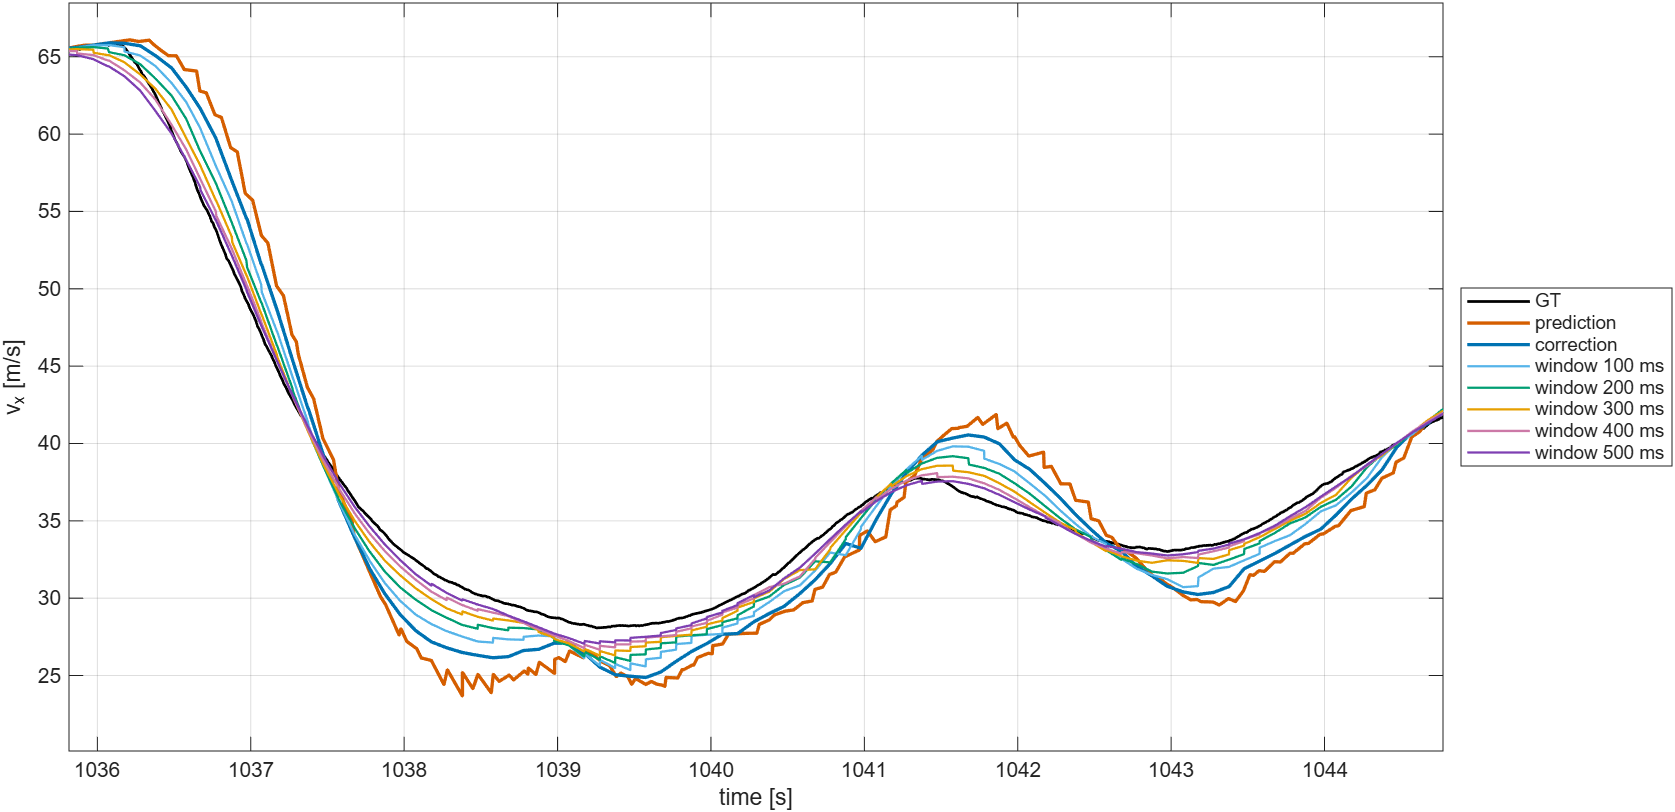
\includegraphics[width=0.76\textwidth]{figures/ch6/rts_lag_noradar_corner.png}}
    \caption{Speed of the opponent estimated with different windows, without the RaDAR.}
    \label{fig:rts_lag_noradar}
\end{figure}

\begin{figure}[!htbp]
    \centering
    \subfloat[RMSE of the speed]{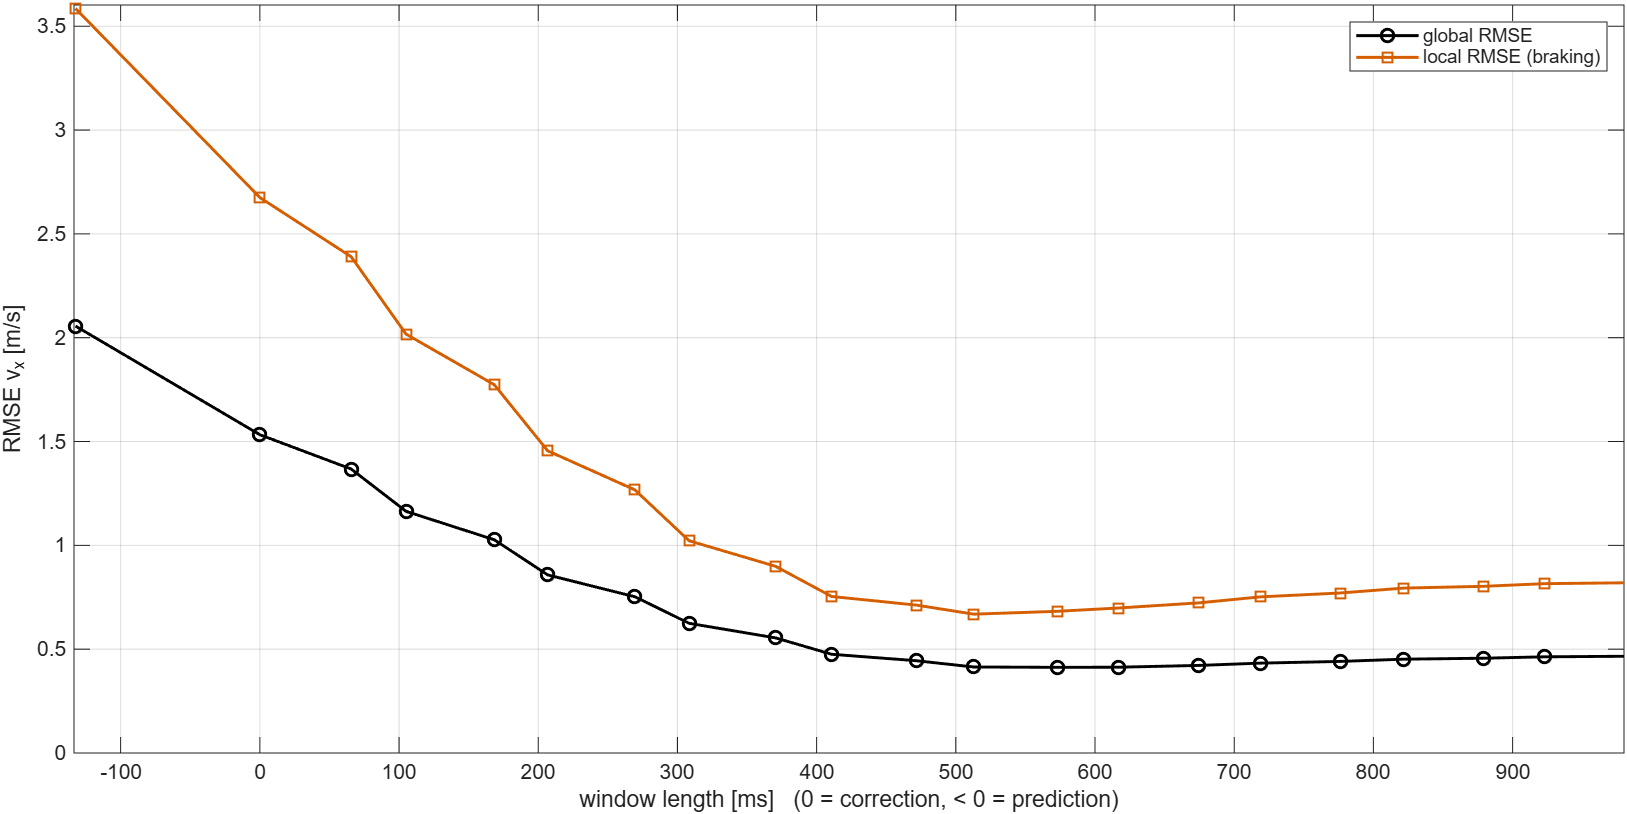
\includegraphics[width=0.76\textwidth]{figures/ch6/rts_rmse_noradar.png}}\\
    \subfloat[Maneuver delay]{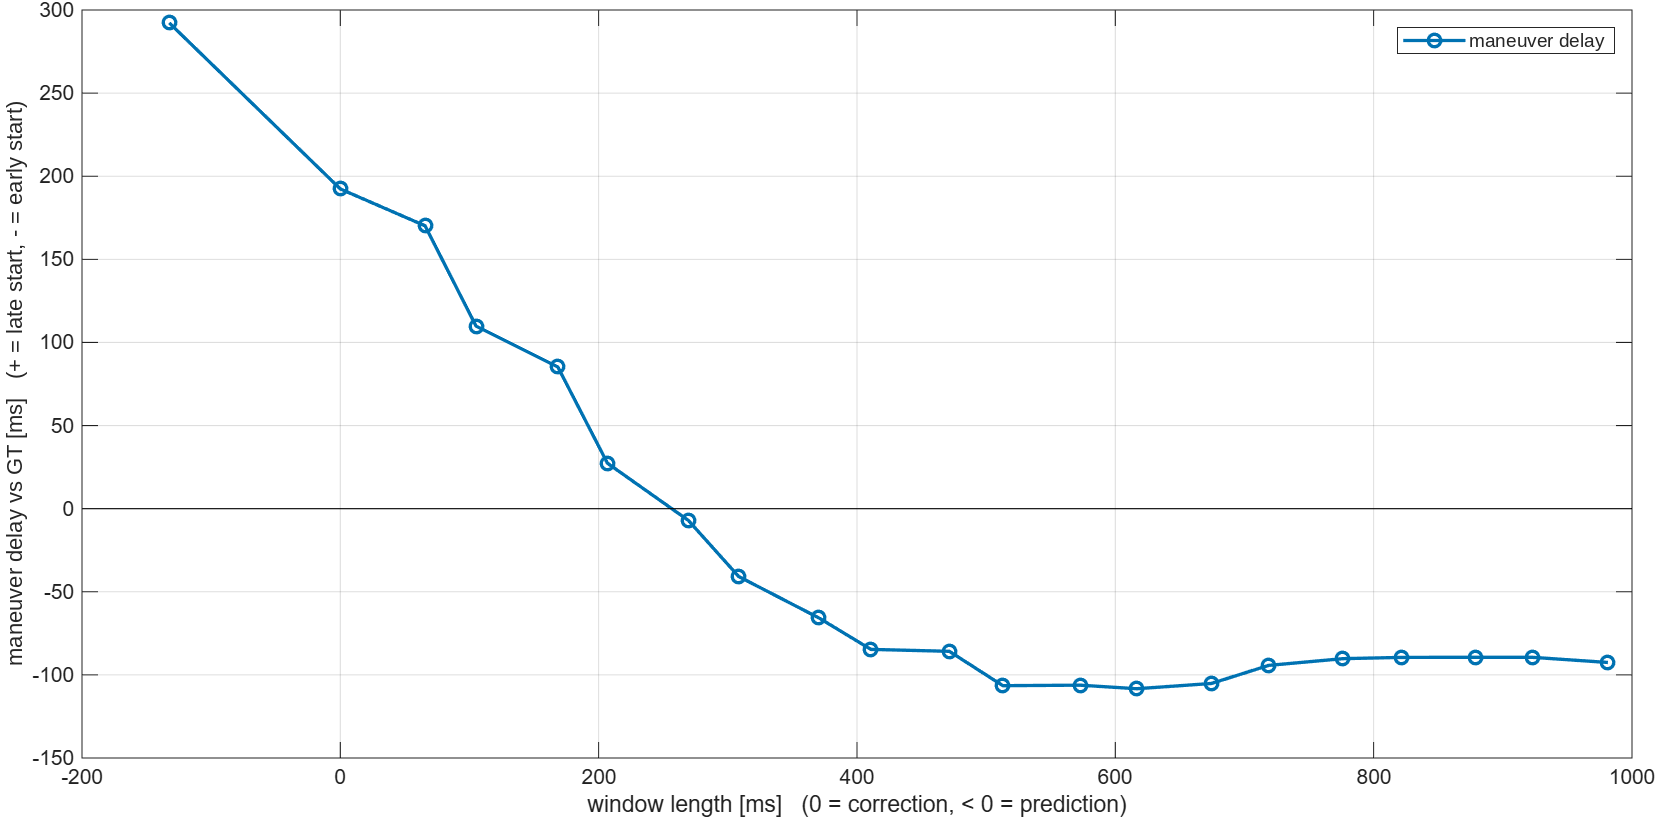
\includegraphics[width=0.76\textwidth]{figures/ch6/rts_delay_noradar.png}}
    \caption{RMSE of the speed and maneuver delay as a function of the window length, without
    the RaDAR.}
    \label{fig:rts_metrics_noradar}
\end{figure}

The results without the RaDAR are reported in Table~\ref{tab:rts_noradar}. The filtered
estimate is less accurate than with all the sensors, with a global RMSE of
\SI{1.533}{m/s} against \SI{0.938}{m/s}, and it starts the maneuvers later, with a median
maneuver delay of $+192$\,ms. Enlarging the window, the future information available to
the smoother increases and, since the forward filter is more uncertain, the smoother
corrects more. The global RMSE keeps decreasing up to about 500--\SI{600}{ms}, with a
reduction of \SI{73}{\percent}. The larger correction, however, also leads to anticipating
the maneuvers. The median maneuver delay becomes negative beyond about \SI{270}{ms}, and
it moves from \SI{-7}{ms} at \SI{269}{ms} to \SI{-41}{ms} at \SI{308}{ms}, \SI{-85}{ms} at
\SI{411}{ms} and \SI{-106}{ms} at \SI{513}{ms}, i.e.\ the effect grows as the window is
enlarged. As shown by the local RMSE, computed isolating the braking maneuvers, this
anticipation eventually degrades the estimate. The local RMSE reaches its minimum of
\SI{0.669}{m/s} at about \SI{500}{ms} and then starts increasing, up to \SI{0.820}{m/s} at
\SI{981}{ms}, i.e.\ beyond this point anticipating the maneuver increases the error.

\begin{table}[!htbp]
\centering
\small
\begin{tabular}{rccccc}
\toprule
Window & \multicolumn{2}{c}{Global RMSE} & \multicolumn{2}{c}{Local RMSE} & Maneuver delay \\
\cmidrule(lr){2-3}\cmidrule(lr){4-5}
[ms] & [m/s] & $\Delta$ [\%] & [m/s] & $\Delta$ [\%] & [ms] \\
\midrule
 $-132$ & 2.056 & $+34.1$ & 3.585 & $+34.0$ & $+292$ \\
      0 & 1.533 & -- & 2.675 & -- & $+192$ \\
    105 & 1.164 & $-24.1$ & 2.017 & $-24.6$ & $+110$ \\
    207 & 0.858 & $-44.0$ & 1.455 & $-45.6$ & $+27$ \\
    308 & 0.625 & $-59.2$ & 1.022 & $-61.8$ & $-41$ \\
    411 & 0.476 & $-68.9$ & 0.754 & $-71.8$ & $-85$ \\
    513 & 0.414 & $-73.0$ & 0.669 & $-75.0$ & $-106$ \\
    617 & 0.413 & $-73.1$ & 0.698 & $-73.9$ & $-108$ \\
    719 & 0.433 & $-71.8$ & 0.752 & $-71.9$ & $-94$ \\
    821 & 0.452 & $-70.5$ & 0.794 & $-70.3$ & $-89$ \\
    981 & 0.466 & $-69.6$ & 0.820 & $-69.3$ & $-93$ \\
\bottomrule
\end{tabular}
\caption{RMSE of the speed and median maneuver delay as a function of the window length, without the RaDAR. $\Delta$ is the variation with respect to the filtered estimate.}
\label{tab:rts_noradar}
\end{table}

\FloatBarrier
\subsection*{Comparison}
\label{subsec:rts_comparison}

Overall, the quality of the estimate of the speed improves in both cases, which justifies
the idea of using an acausal approach to improve the estimate of the state of the
opponent. The two cases are compared in Table~\ref{tab:rts_radar_noradar}.

\begin{table}[!htbp]
\centering
\small
\begin{tabular}{rcccccc}
\toprule
Window & \multicolumn{2}{c}{Global RMSE [m/s]} & \multicolumn{2}{c}{Local RMSE [m/s]} & \multicolumn{2}{c}{Maneuver delay [ms]} \\
\cmidrule(lr){2-3}\cmidrule(lr){4-5}\cmidrule(lr){6-7}
[ms] & RaDAR & No RaDAR & RaDAR & No RaDAR & RaDAR & No RaDAR \\
\midrule
$\approx -100$  & 1.177 & 2.056 & 2.218 & 3.585 & $+99$ & $+292$ \\
0               & 0.938 & 1.533 & 1.724 & 2.675 & $+19$ & $+192$ \\
$\approx 100$   & 0.815 & 1.164 & 1.467 & 2.017 & $-19$ & $+110$ \\
$\approx 200$   & 0.671 & 0.858 & 1.164 & 1.455 & $-61$ & $+27$ \\
$\approx 300$   & 0.646 & 0.625 & 1.114 & 1.022 & $-62$ & $-41$ \\
$\approx 400$   & 0.647 & 0.476 & 1.113 & 0.754 & $-62$ & $-85$ \\
$\approx 500$   & 0.648 & 0.414 & 1.113 & 0.669 & $-62$ & $-106$ \\
\bottomrule
\end{tabular}
\caption{RMSE of the speed and median maneuver delay as a function of the window length, with and
without the RaDAR.}
\label{tab:rts_radar_noradar}
\end{table}

The window length is fixed at about \SI{300}{ms} as a compromise between the two cases.
With the RaDAR, the improvement saturates at about \SI{300}{ms}, so that a longer window
brings no further benefit. Without it, the RMSE keeps decreasing with longer windows, but
the anticipation of the maneuvers grows with the window, and beyond about \SI{500}{ms} the
local RMSE increases again. A window of \SI{300}{ms} therefore keeps the anticipation
limited in both cases, at the cost of a higher RMSE than the minimum reachable without the
RaDAR.

Fixing the window at \SI{300}{ms}, Fig.~\ref{fig:rts_radar_noradar}
shows the comparison of the speed and of the acceleration estimated with and without the
RaDAR measurements. The orange lines are the smoothed (solid) and the causal (dashed)
estimates with the RaDAR measurements, while the blue ones are the same estimates without
the RaDAR measurements. As shown in the figure, in both cases the quality of the estimate
of the speed, and also of the acceleration, improves significantly.

\begin{figure}[H]
    \centering
    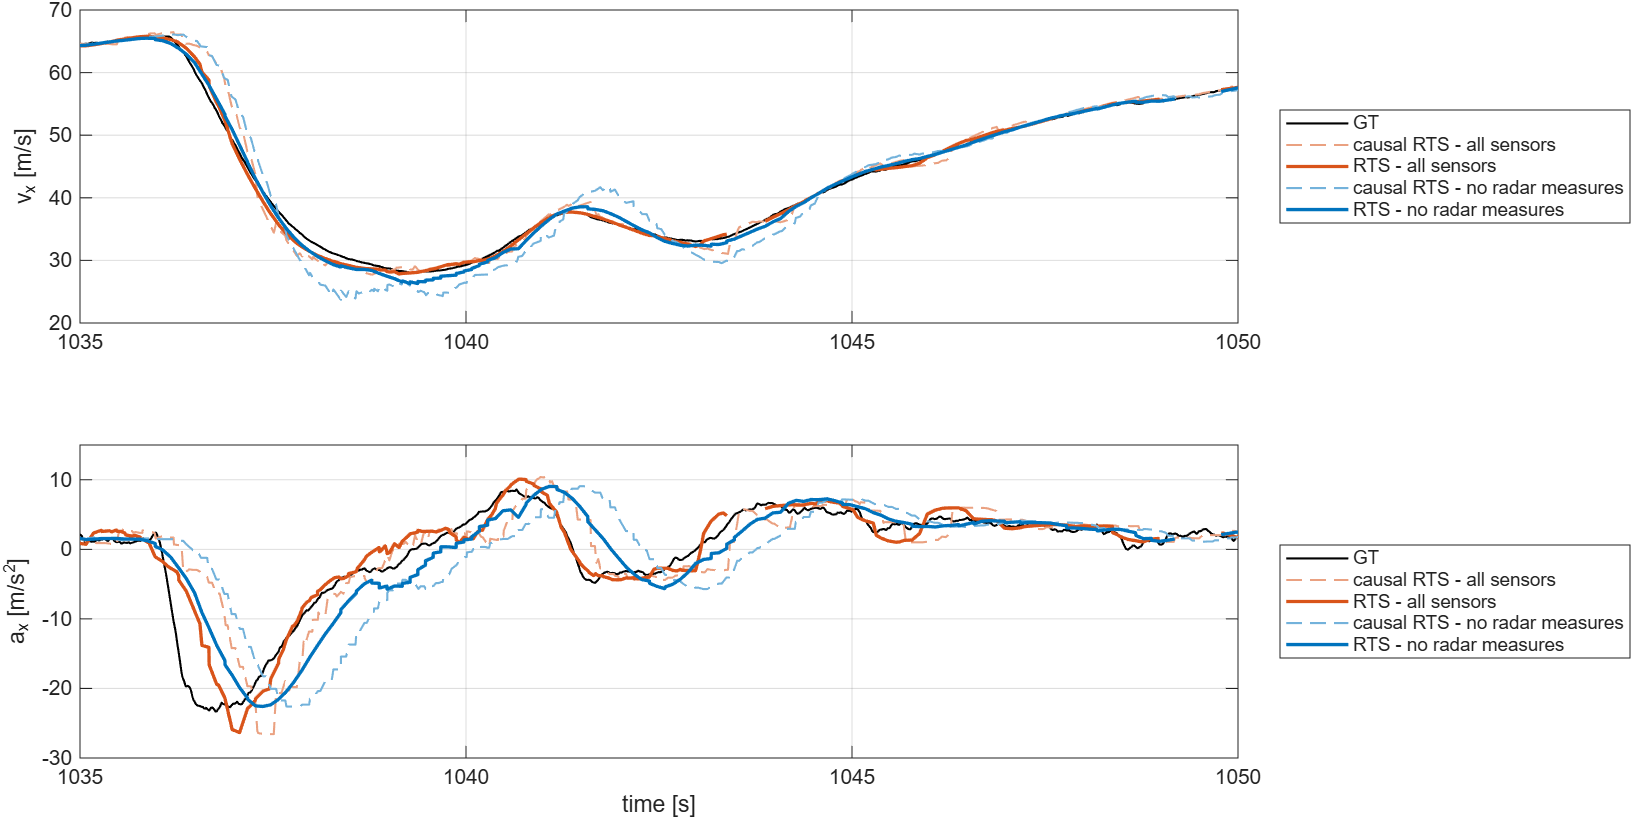
\includegraphics[width=0.85\textwidth]{figures/ch6/rts_radar_vs_noradar.png}
    \caption{Speed and acceleration estimated with and without the RaDAR, window of
    \SI{300}{ms}.}
    \label{fig:rts_radar_noradar}
\end{figure}

At \SI{300}{ms}, the smoothed estimate without the RaDAR reaches a global RMSE of
\SI{0.625}{m/s} and a local one of \SI{1.022}{m/s}, against \SI{0.646}{m/s} and
\SI{1.114}{m/s} with all the sensors. The most important result is therefore that, even in
the absence of direct measurements of the speed, the smoother provides a reliable estimate
of the speed of the opponent.

% =====================================================================
\section{Combination with the Q Feed-Forward}
\label{sec:rts_qff}

\TODO{Combination of the RTS smoother with the feed-forward process noise of
Chapter~\ref{ch:qff}. The smoother in series with the feed-forward approach could reduce
the effect of the noise of the jerk estimate and of the false activations of the maneuver
flag. Formulation, implementation and results.}
